% Created by tikzDevice version 0.12
% !TEX encoding = UTF-8 Unicode
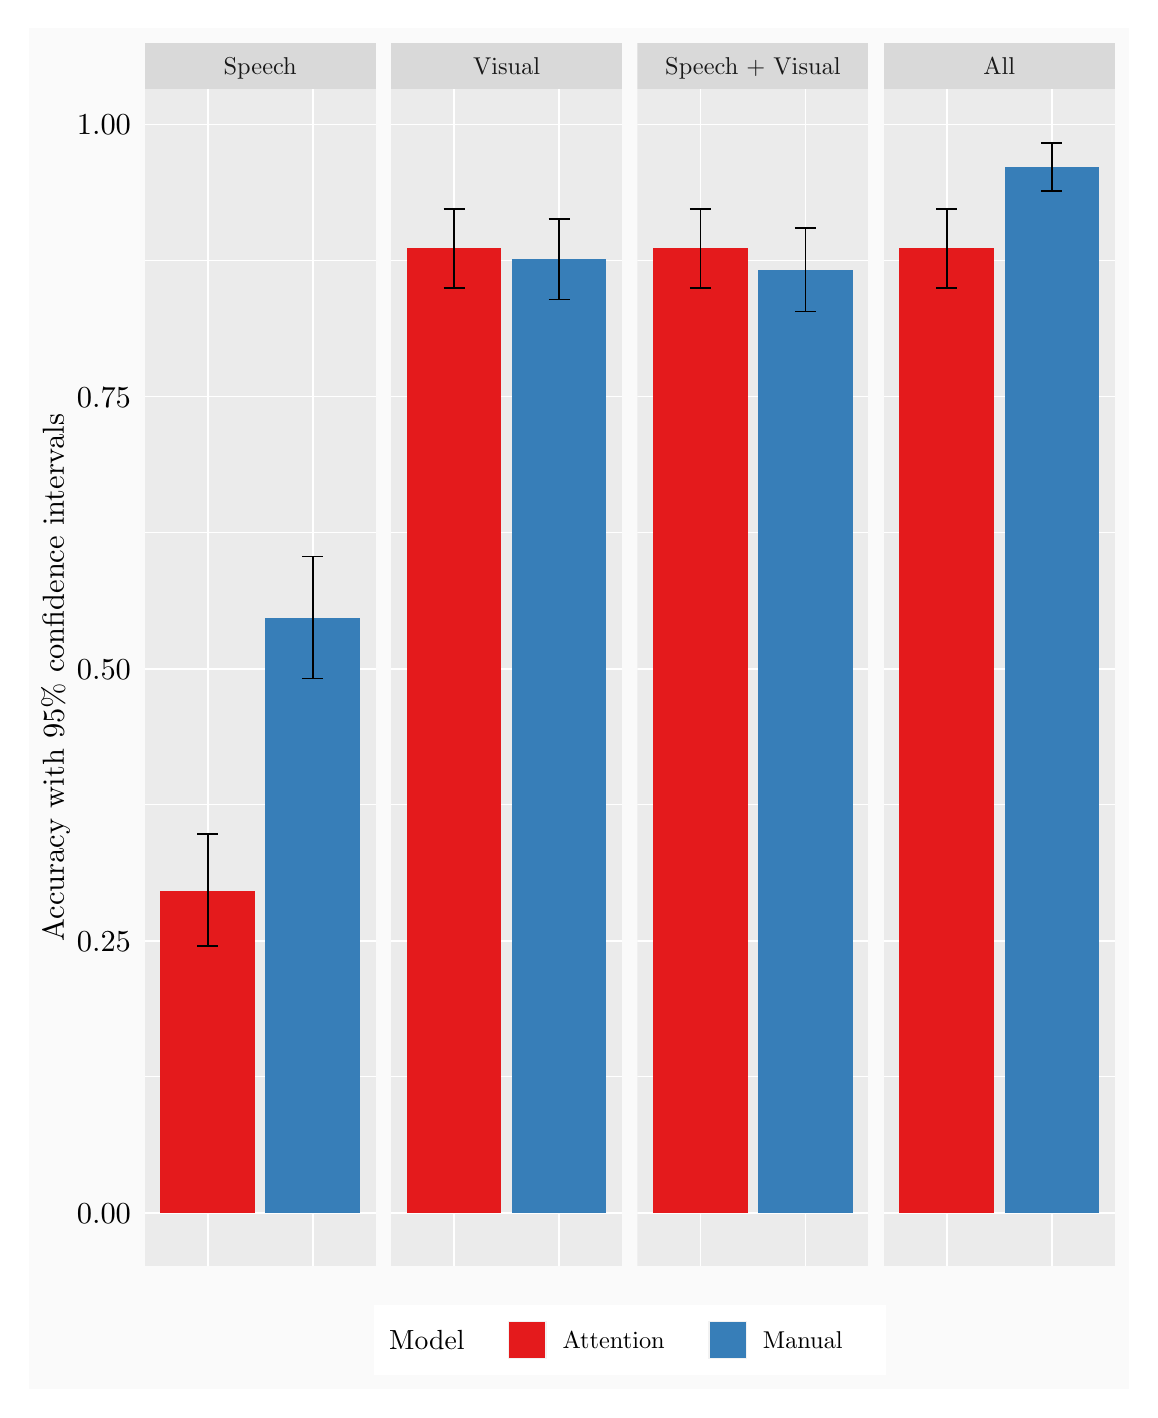
\begin{tikzpicture}[x=1pt,y=1pt]
\definecolor{fillColor}{RGB}{255,255,255}
\path[use as bounding box,fill=fillColor,fill opacity=0.00] (0,0) rectangle (398.34,492.35);
\begin{scope}
\path[clip] (  0.00,  0.00) rectangle (398.34,492.35);
\definecolor{drawColor}{RGB}{255,255,255}
\definecolor{fillColor}{gray}{0.98}

\path[draw=drawColor,line width= 0.6pt,line join=round,line cap=round,fill=fillColor] (  0.00,  0.00) rectangle (398.34,492.35);
\end{scope}
\begin{scope}
\path[clip] ( 42.27, 44.70) rectangle (125.79,470.04);
\definecolor{fillColor}{gray}{0.92}

\path[fill=fillColor] ( 42.27, 44.70) rectangle (125.79,470.04);
\definecolor{drawColor}{RGB}{255,255,255}

\path[draw=drawColor,line width= 0.3pt,line join=round] ( 42.27,113.21) --
	(125.79,113.21);

\path[draw=drawColor,line width= 0.3pt,line join=round] ( 42.27,211.55) --
	(125.79,211.55);

\path[draw=drawColor,line width= 0.3pt,line join=round] ( 42.27,309.89) --
	(125.79,309.89);

\path[draw=drawColor,line width= 0.3pt,line join=round] ( 42.27,408.23) --
	(125.79,408.23);

\path[draw=drawColor,line width= 0.6pt,line join=round] ( 42.27, 64.04) --
	(125.79, 64.04);

\path[draw=drawColor,line width= 0.6pt,line join=round] ( 42.27,162.38) --
	(125.79,162.38);

\path[draw=drawColor,line width= 0.6pt,line join=round] ( 42.27,260.72) --
	(125.79,260.72);

\path[draw=drawColor,line width= 0.6pt,line join=round] ( 42.27,359.06) --
	(125.79,359.06);

\path[draw=drawColor,line width= 0.6pt,line join=round] ( 42.27,457.40) --
	(125.79,457.40);

\path[draw=drawColor,line width= 0.6pt,line join=round] ( 65.05, 44.70) --
	( 65.05,470.04);

\path[draw=drawColor,line width= 0.6pt,line join=round] (103.01, 44.70) --
	(103.01,470.04);
\definecolor{fillColor}{RGB}{228,26,28}

\path[fill=fillColor] ( 47.97, 64.04) rectangle ( 82.13,180.47);
\definecolor{fillColor}{RGB}{55,126,184}

\path[fill=fillColor] ( 85.93, 64.04) rectangle (120.09,279.20);
\definecolor{drawColor}{RGB}{0,0,0}

\path[draw=drawColor,line width= 0.6pt,line join=round] ( 61.25,200.93) --
	( 68.84,200.93);

\path[draw=drawColor,line width= 0.6pt,line join=round] ( 65.05,200.93) --
	( 65.05,160.41);

\path[draw=drawColor,line width= 0.6pt,line join=round] ( 61.25,160.41) --
	( 68.84,160.41);

\path[draw=drawColor,line width= 0.6pt,line join=round] ( 99.21,301.23) --
	(106.81,301.23);

\path[draw=drawColor,line width= 0.6pt,line join=round] (103.01,301.23) --
	(103.01,257.18);

\path[draw=drawColor,line width= 0.6pt,line join=round] ( 99.21,257.18) --
	(106.81,257.18);
\end{scope}
\begin{scope}
\path[clip] (131.29, 44.70) rectangle (214.80,470.04);
\definecolor{fillColor}{gray}{0.92}

\path[fill=fillColor] (131.29, 44.70) rectangle (214.80,470.04);
\definecolor{drawColor}{RGB}{255,255,255}

\path[draw=drawColor,line width= 0.3pt,line join=round] (131.29,113.21) --
	(214.80,113.21);

\path[draw=drawColor,line width= 0.3pt,line join=round] (131.29,211.55) --
	(214.80,211.55);

\path[draw=drawColor,line width= 0.3pt,line join=round] (131.29,309.89) --
	(214.80,309.89);

\path[draw=drawColor,line width= 0.3pt,line join=round] (131.29,408.23) --
	(214.80,408.23);

\path[draw=drawColor,line width= 0.6pt,line join=round] (131.29, 64.04) --
	(214.80, 64.04);

\path[draw=drawColor,line width= 0.6pt,line join=round] (131.29,162.38) --
	(214.80,162.38);

\path[draw=drawColor,line width= 0.6pt,line join=round] (131.29,260.72) --
	(214.80,260.72);

\path[draw=drawColor,line width= 0.6pt,line join=round] (131.29,359.06) --
	(214.80,359.06);

\path[draw=drawColor,line width= 0.6pt,line join=round] (131.29,457.40) --
	(214.80,457.40);

\path[draw=drawColor,line width= 0.6pt,line join=round] (154.07, 44.70) --
	(154.07,470.04);

\path[draw=drawColor,line width= 0.6pt,line join=round] (192.03, 44.70) --
	(192.03,470.04);
\definecolor{fillColor}{RGB}{228,26,28}

\path[fill=fillColor] (136.98, 64.04) rectangle (171.15,412.55);
\definecolor{fillColor}{RGB}{55,126,184}

\path[fill=fillColor] (174.94, 64.04) rectangle (209.11,408.62);
\definecolor{drawColor}{RGB}{0,0,0}

\path[draw=drawColor,line width= 0.6pt,line join=round] (150.27,426.71) --
	(157.86,426.71);

\path[draw=drawColor,line width= 0.6pt,line join=round] (154.07,426.71) --
	(154.07,398.39);

\path[draw=drawColor,line width= 0.6pt,line join=round] (150.27,398.39) --
	(157.86,398.39);

\path[draw=drawColor,line width= 0.6pt,line join=round] (188.23,423.17) --
	(195.82,423.17);

\path[draw=drawColor,line width= 0.6pt,line join=round] (192.03,423.17) --
	(192.03,394.06);

\path[draw=drawColor,line width= 0.6pt,line join=round] (188.23,394.06) --
	(195.82,394.06);
\end{scope}
\begin{scope}
\path[clip] (220.30, 44.70) rectangle (303.82,470.04);
\definecolor{fillColor}{gray}{0.92}

\path[fill=fillColor] (220.30, 44.70) rectangle (303.82,470.04);
\definecolor{drawColor}{RGB}{255,255,255}

\path[draw=drawColor,line width= 0.3pt,line join=round] (220.30,113.21) --
	(303.82,113.21);

\path[draw=drawColor,line width= 0.3pt,line join=round] (220.30,211.55) --
	(303.82,211.55);

\path[draw=drawColor,line width= 0.3pt,line join=round] (220.30,309.89) --
	(303.82,309.89);

\path[draw=drawColor,line width= 0.3pt,line join=round] (220.30,408.23) --
	(303.82,408.23);

\path[draw=drawColor,line width= 0.6pt,line join=round] (220.30, 64.04) --
	(303.82, 64.04);

\path[draw=drawColor,line width= 0.6pt,line join=round] (220.30,162.38) --
	(303.82,162.38);

\path[draw=drawColor,line width= 0.6pt,line join=round] (220.30,260.72) --
	(303.82,260.72);

\path[draw=drawColor,line width= 0.6pt,line join=round] (220.30,359.06) --
	(303.82,359.06);

\path[draw=drawColor,line width= 0.6pt,line join=round] (220.30,457.40) --
	(303.82,457.40);

\path[draw=drawColor,line width= 0.6pt,line join=round] (243.08, 44.70) --
	(243.08,470.04);

\path[draw=drawColor,line width= 0.6pt,line join=round] (281.04, 44.70) --
	(281.04,470.04);
\definecolor{fillColor}{RGB}{228,26,28}

\path[fill=fillColor] (226.00, 64.04) rectangle (260.17,412.55);
\definecolor{fillColor}{RGB}{55,126,184}

\path[fill=fillColor] (263.96, 64.04) rectangle (298.13,404.69);
\definecolor{drawColor}{RGB}{0,0,0}

\path[draw=drawColor,line width= 0.6pt,line join=round] (239.29,426.71) --
	(246.88,426.71);

\path[draw=drawColor,line width= 0.6pt,line join=round] (243.08,426.71) --
	(243.08,398.39);

\path[draw=drawColor,line width= 0.6pt,line join=round] (239.29,398.39) --
	(246.88,398.39);

\path[draw=drawColor,line width= 0.6pt,line join=round] (277.25,420.03) --
	(284.84,420.03);

\path[draw=drawColor,line width= 0.6pt,line join=round] (281.04,420.03) --
	(281.04,389.74);

\path[draw=drawColor,line width= 0.6pt,line join=round] (277.25,389.74) --
	(284.84,389.74);
\end{scope}
\begin{scope}
\path[clip] (309.32, 44.70) rectangle (392.84,470.04);
\definecolor{fillColor}{gray}{0.92}

\path[fill=fillColor] (309.32, 44.70) rectangle (392.84,470.04);
\definecolor{drawColor}{RGB}{255,255,255}

\path[draw=drawColor,line width= 0.3pt,line join=round] (309.32,113.21) --
	(392.84,113.21);

\path[draw=drawColor,line width= 0.3pt,line join=round] (309.32,211.55) --
	(392.84,211.55);

\path[draw=drawColor,line width= 0.3pt,line join=round] (309.32,309.89) --
	(392.84,309.89);

\path[draw=drawColor,line width= 0.3pt,line join=round] (309.32,408.23) --
	(392.84,408.23);

\path[draw=drawColor,line width= 0.6pt,line join=round] (309.32, 64.04) --
	(392.84, 64.04);

\path[draw=drawColor,line width= 0.6pt,line join=round] (309.32,162.38) --
	(392.84,162.38);

\path[draw=drawColor,line width= 0.6pt,line join=round] (309.32,260.72) --
	(392.84,260.72);

\path[draw=drawColor,line width= 0.6pt,line join=round] (309.32,359.06) --
	(392.84,359.06);

\path[draw=drawColor,line width= 0.6pt,line join=round] (309.32,457.40) --
	(392.84,457.40);

\path[draw=drawColor,line width= 0.6pt,line join=round] (332.10, 44.70) --
	(332.10,470.04);

\path[draw=drawColor,line width= 0.6pt,line join=round] (370.06, 44.70) --
	(370.06,470.04);
\definecolor{fillColor}{RGB}{228,26,28}

\path[fill=fillColor] (315.02, 64.04) rectangle (349.18,412.55);
\definecolor{fillColor}{RGB}{55,126,184}

\path[fill=fillColor] (352.98, 64.04) rectangle (387.14,442.05);
\definecolor{drawColor}{RGB}{0,0,0}

\path[draw=drawColor,line width= 0.6pt,line join=round] (328.30,426.71) --
	(335.90,426.71);

\path[draw=drawColor,line width= 0.6pt,line join=round] (332.10,426.71) --
	(332.10,398.39);

\path[draw=drawColor,line width= 0.6pt,line join=round] (328.30,398.39) --
	(335.90,398.39);

\path[draw=drawColor,line width= 0.6pt,line join=round] (366.27,450.71) --
	(373.86,450.71);

\path[draw=drawColor,line width= 0.6pt,line join=round] (370.06,450.71) --
	(370.06,433.40);

\path[draw=drawColor,line width= 0.6pt,line join=round] (366.27,433.40) --
	(373.86,433.40);
\end{scope}
\begin{scope}
\path[clip] ( 42.27,470.04) rectangle (125.79,486.85);
\definecolor{fillColor}{gray}{0.85}

\path[fill=fillColor] ( 42.27,470.04) rectangle (125.79,486.85);
\definecolor{drawColor}{gray}{0.10}

\node[text=drawColor,anchor=base,inner sep=0pt, outer sep=0pt, scale=  0.88] at ( 84.03,475.41) {Speech};
\end{scope}
\begin{scope}
\path[clip] (131.29,470.04) rectangle (214.80,486.85);
\definecolor{fillColor}{gray}{0.85}

\path[fill=fillColor] (131.29,470.04) rectangle (214.80,486.85);
\definecolor{drawColor}{gray}{0.10}

\node[text=drawColor,anchor=base,inner sep=0pt, outer sep=0pt, scale=  0.88] at (173.05,475.41) {Visual};
\end{scope}
\begin{scope}
\path[clip] (220.30,470.04) rectangle (303.82,486.85);
\definecolor{fillColor}{gray}{0.85}

\path[fill=fillColor] (220.30,470.04) rectangle (303.82,486.85);
\definecolor{drawColor}{gray}{0.10}

\node[text=drawColor,anchor=base,inner sep=0pt, outer sep=0pt, scale=  0.88] at (262.06,475.41) {Speech + Visual};
\end{scope}
\begin{scope}
\path[clip] (309.32,470.04) rectangle (392.84,486.85);
\definecolor{fillColor}{gray}{0.85}

\path[fill=fillColor] (309.32,470.04) rectangle (392.84,486.85);
\definecolor{drawColor}{gray}{0.10}

\node[text=drawColor,anchor=base,inner sep=0pt, outer sep=0pt, scale=  0.88] at (351.08,475.41) {All};
\end{scope}
\begin{scope}
\path[clip] (  0.00,  0.00) rectangle (398.34,492.35);
\definecolor{drawColor}{RGB}{0,0,0}

\node[text=drawColor,anchor=base east,inner sep=0pt, outer sep=0pt, scale=  1.10] at ( 37.32, 60.25) {0.00};

\node[text=drawColor,anchor=base east,inner sep=0pt, outer sep=0pt, scale=  1.10] at ( 37.32,158.59) {0.25};

\node[text=drawColor,anchor=base east,inner sep=0pt, outer sep=0pt, scale=  1.10] at ( 37.32,256.93) {0.50};

\node[text=drawColor,anchor=base east,inner sep=0pt, outer sep=0pt, scale=  1.10] at ( 37.32,355.27) {0.75};

\node[text=drawColor,anchor=base east,inner sep=0pt, outer sep=0pt, scale=  1.10] at ( 37.32,453.61) {1.00};
\end{scope}
\begin{scope}
\path[clip] (  0.00,  0.00) rectangle (398.34,492.35);
\definecolor{drawColor}{RGB}{0,0,0}

\node[text=drawColor,rotate= 90.00,anchor=base,inner sep=0pt, outer sep=0pt, scale=  1.10] at ( 13.08,257.37) {Accuracy with 95\% confidence intervals};
\end{scope}
\begin{scope}
\path[clip] (  0.00,  0.00) rectangle (398.34,492.35);
\definecolor{fillColor}{RGB}{255,255,255}

\path[fill=fillColor] (125.12,  5.50) rectangle (309.99, 30.95);
\end{scope}
\begin{scope}
\path[clip] (  0.00,  0.00) rectangle (398.34,492.35);
\definecolor{drawColor}{RGB}{0,0,0}

\node[text=drawColor,anchor=base west,inner sep=0pt, outer sep=0pt, scale=  1.00] at (130.62, 14.78) {Model};
\end{scope}
\begin{scope}
\path[clip] (  0.00,  0.00) rectangle (398.34,492.35);
\definecolor{drawColor}{RGB}{255,255,255}
\definecolor{fillColor}{gray}{0.95}

\path[draw=drawColor,line width= 0.6pt,line join=round,line cap=round,fill=fillColor] (173.34, 11.00) rectangle (187.79, 25.45);
\end{scope}
\begin{scope}
\path[clip] (  0.00,  0.00) rectangle (398.34,492.35);
\definecolor{fillColor}{RGB}{228,26,28}

\path[fill=fillColor] (174.05, 11.71) rectangle (187.08, 24.74);
\end{scope}
\begin{scope}
\path[clip] (  0.00,  0.00) rectangle (398.34,492.35);
\definecolor{drawColor}{RGB}{255,255,255}
\definecolor{fillColor}{gray}{0.95}

\path[draw=drawColor,line width= 0.6pt,line join=round,line cap=round,fill=fillColor] (245.69, 11.00) rectangle (260.15, 25.45);
\end{scope}
\begin{scope}
\path[clip] (  0.00,  0.00) rectangle (398.34,492.35);
\definecolor{fillColor}{RGB}{55,126,184}

\path[fill=fillColor] (246.41, 11.71) rectangle (259.44, 24.74);
\end{scope}
\begin{scope}
\path[clip] (  0.00,  0.00) rectangle (398.34,492.35);
\definecolor{drawColor}{RGB}{0,0,0}

\node[text=drawColor,anchor=base west,inner sep=0pt, outer sep=0pt, scale=  0.88] at (193.29, 15.20) {Attention};
\end{scope}
\begin{scope}
\path[clip] (  0.00,  0.00) rectangle (398.34,492.35);
\definecolor{drawColor}{RGB}{0,0,0}

\node[text=drawColor,anchor=base west,inner sep=0pt, outer sep=0pt, scale=  0.88] at (265.65, 15.20) {Manual};
\end{scope}
\end{tikzpicture}
